% =============================================================================
% Day 7: Databricks Jobs and Workflows - Complete Guide
% Databricks Color Theme LaTeX Beamer Presentation
% =============================================================================

\documentclass[aspectratio=169]{beamer}

% -----------------------------------------------------------------------------
% PACKAGES
% -----------------------------------------------------------------------------
\usepackage{tikz}
\usepackage{graphicx}
\usepackage{hyperref}
\usepackage{xcolor}
\usepackage{listings}
\usepackage{fontawesome5}
\usepackage{booktabs}
\usepackage{array}
\usepackage{multirow}
\usepackage{colortbl}

% -----------------------------------------------------------------------------
% DATABRICKS COLOR DEFINITIONS
% -----------------------------------------------------------------------------
\definecolor{databricksBlue}{RGB}{41, 49, 66}
\definecolor{databricksRed}{RGB}{220, 53, 69}
\definecolor{databricksYellow}{RGB}{255, 193, 7}
\definecolor{databricksGreen}{RGB}{76, 175, 80}
\definecolor{databricksGray}{RGB}{128, 128, 128}
\definecolor{databricksLightGray}{RGB}{245, 245, 245}
\definecolor{databricksWhite}{RGB}{255, 255, 255}
\definecolor{bronzeColor}{RGB}{205, 127, 50}
\definecolor{silverColor}{RGB}{192, 192, 192}
\definecolor{goldColor}{RGB}{255, 215, 0}

% -----------------------------------------------------------------------------
% BEAMER THEME CONFIGURATION
% -----------------------------------------------------------------------------
\usetheme{default}
\usecolortheme{default}

% Remove navigation symbols
\setbeamertemplate{navigation symbols}{}

% Frame title
\setbeamercolor{frametitle}{fg=databricksWhite, bg=databricksBlue}
\setbeamerfont{frametitle}{size=\large, series=\bfseries}

% Title page colors
\setbeamercolor{title}{fg=databricksWhite}
\setbeamercolor{subtitle}{fg=databricksLightGray}
\setbeamercolor{author}{fg=databricksWhite}
\setbeamercolor{institute}{fg=databricksLightGray}
\setbeamercolor{date}{fg=databricksYellow}

% Item colors
\setbeamercolor{itemize item}{fg=databricksBlue}
\setbeamercolor{itemize subitem}{fg=databricksRed}
\setbeamercolor{itemize subsubitem}{fg=databricksGreen}

\setbeamertemplate{itemize item}{\textcolor{databricksBlue}{$\bullet$}}
\setbeamertemplate{itemize subitem}{\textcolor{databricksRed}{$\triangleright$}}
\setbeamertemplate{itemize subsubitem}{\textcolor{databricksGreen}{$\circ$}}

% Block colors
\setbeamercolor{block title}{fg=databricksWhite, bg=databricksBlue}
\setbeamercolor{block body}{fg=databricksBlue, bg=databricksLightGray}

% -----------------------------------------------------------------------------
% LISTINGS CONFIGURATION
% -----------------------------------------------------------------------------
\lstset{
    basicstyle=\tiny\ttfamily,
    backgroundcolor=\color{databricksLightGray},
    frame=single,
    framerule=0.5pt,
    rulecolor=\color{databricksBlue},
    breaklines=true,
    showstringspaces=false,
    keywordstyle=\color{databricksBlue}\bfseries,
    stringstyle=\color{databricksGreen},
    commentstyle=\color{databricksGray}\itshape,
    numbers=none,
    xleftmargin=2pt,
    xrightmargin=2pt,
    aboveskip=3pt,
    belowskip=3pt
}

% -----------------------------------------------------------------------------
% FOOTER CONFIGURATION
% -----------------------------------------------------------------------------
\setbeamertemplate{footline}{
    \leavevmode%
    \hbox{%
        \begin{beamercolorbox}[wd=.33\paperwidth,ht=2.5ex,dp=1ex,left]{author in head/foot}%
            \usebeamerfont{author in head/foot}\hspace*{2ex}%
            \href{https://easy-ai-labs.lovable.app/}{\textcolor{databricksBlue}{Easy AI Labs}}
        \end{beamercolorbox}%
        \begin{beamercolorbox}[wd=.34\paperwidth,ht=2.5ex,dp=1ex,center]{title in head/foot}%
            \usebeamerfont{title in head/foot}%
            \href{https://www.linkedin.com/in/yashkavaiya}{\textcolor{databricksBlue}{Yash Kavaiya}}
        \end{beamercolorbox}%
        \begin{beamercolorbox}[wd=.33\paperwidth,ht=2.5ex,dp=1ex,right]{date in head/foot}%
            \usebeamerfont{date in head/foot}%
            \href{https://www.linkedin.com/company/genai-guru}{\textcolor{databricksBlue}{Gen AI Guru}}\hspace*{2ex}
            \insertframenumber{}/\inserttotalframenumber\hspace*{2ex}
        \end{beamercolorbox}%
    }%
    \vskip0pt%
}

% -----------------------------------------------------------------------------
% TITLE PAGE TEMPLATE
% -----------------------------------------------------------------------------
\defbeamertemplate*{title page}{customized}[1][]
{
    \begin{tikzpicture}[remember picture,overlay]
        \fill[databricksBlue] (current page.north west) rectangle (current page.south east);
    \end{tikzpicture}
    \vfill
    \begin{center}
        {\usebeamerfont{title}\usebeamercolor[fg]{title}\LARGE\textbf{\inserttitle}\par}
        \vskip0.5em
        {\usebeamerfont{subtitle}\usebeamercolor[fg]{subtitle}\large\insertsubtitle\par}
        \vskip1.5em
        {\usebeamerfont{author}\usebeamercolor[fg]{author}\insertauthor\par}
        \vskip0.5em
        {\usebeamerfont{institute}\usebeamercolor[fg]{institute}\insertinstitute\par}
        \vskip1em
        {\usebeamerfont{date}\usebeamercolor[fg]{date}\insertdate\par}
    \end{center}
    \vfill
}

% -----------------------------------------------------------------------------
% DOCUMENT METADATA
% -----------------------------------------------------------------------------
\title{Databricks Jobs \& Workflows}
\subtitle{Complete Guide - Day 7}
\author{Yash Kavaiya}
\institute{Databricks 14-Days AI Challenge}
\date{\today}

% =============================================================================
% DOCUMENT BEGIN
% =============================================================================
\begin{document}

% -----------------------------------------------------------------------------
% TITLE SLIDE
% -----------------------------------------------------------------------------
\begin{frame}[plain]
    \titlepage
\end{frame}

% -----------------------------------------------------------------------------
% TABLE OF CONTENTS
% -----------------------------------------------------------------------------
\begin{frame}{Agenda}
    \begin{columns}[T]
        \begin{column}{0.48\textwidth}
            \begin{itemize}
                \item \textcolor{databricksBlue}{\textbf{Introduction to Databricks Jobs}}
                \item \textcolor{databricksBlue}{\textbf{Jobs vs Notebooks}}
                \item \textcolor{databricksBlue}{\textbf{Multi-Task Workflows}}
                \item \textcolor{databricksBlue}{\textbf{Parameters \& Widgets}}
            \end{itemize}
        \end{column}
        \begin{column}{0.48\textwidth}
            \begin{itemize}
                \item \textcolor{databricksBlue}{\textbf{Scheduling Jobs}}
                \item \textcolor{databricksBlue}{\textbf{Error Handling \& Retries}}
                \item \textcolor{databricksBlue}{\textbf{Bronze$\rightarrow$Silver$\rightarrow$Gold Pipeline}}
                \item \textcolor{databricksBlue}{\textbf{Best Practices}}
            \end{itemize}
        \end{column}
    \end{columns}
\end{frame}

% =============================================================================
% SECTION 1: INTRODUCTION TO DATABRICKS JOBS
% =============================================================================
\begin{frame}{What is a Databricks Job?}
    \begin{block}{Definition}
        A \textbf{Databricks Job} is a mechanism to run data processing workloads in a scheduled, automated, and production-ready manner.
    \end{block}
    
    \vspace{0.5em}
    
    \begin{columns}[T]
        \begin{column}{0.55\textwidth}
            \textcolor{databricksBlue}{\textbf{Simple Analogy:}}
            \begin{itemize}
                \item \textcolor{databricksRed}{$\triangleright$} \textbf{Notebook} = Manually cooking a meal step by step
                \item \textcolor{databricksGreen}{$\triangleright$} \textbf{Job} = Automated cooking machine that prepares meals at scheduled times
            \end{itemize}
        \end{column}
        \begin{column}{0.42\textwidth}
            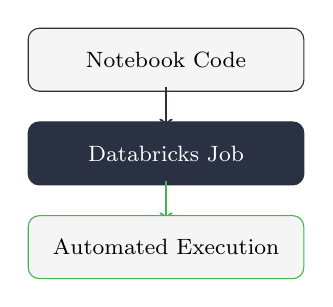
\begin{tikzpicture}[scale=0.7]
                \node[draw=databricksBlue, fill=databricksLightGray, rounded corners, minimum width=3.5cm, minimum height=0.8cm] at (0,2) {\footnotesize Notebook Code};
                \draw[->, thick, databricksBlue] (0,1.5) -- (0,0.8);
                \node[draw=databricksBlue, fill=databricksBlue, text=white, rounded corners, minimum width=3.5cm, minimum height=0.8cm] at (0,0.3) {\footnotesize Databricks Job};
                \draw[->, thick, databricksGreen] (0,-0.2) -- (0,-0.9);
                \node[draw=databricksGreen, fill=databricksLightGray, rounded corners, minimum width=3.5cm, minimum height=0.8cm] at (0,-1.4) {\footnotesize Automated Execution};
            \end{tikzpicture}
        \end{column}
    \end{columns}
\end{frame}

% -----------------------------------------------------------------------------
\begin{frame}{Why Do We Need Jobs?}
    \begin{columns}[T]
        \begin{column}{0.48\textwidth}
            \textcolor{databricksBlue}{\textbf{Common Requirements:}}
            \begin{itemize}
                \item Run transformations at specific times
                    \begin{itemize}
                        \item \textcolor{databricksRed}{$\triangleright$} E.g., daily at 2 AM when load is low
                    \end{itemize}
                \item Ensure reliable processing
                    \begin{itemize}
                        \item \textcolor{databricksRed}{$\triangleright$} Without manual intervention
                    \end{itemize}
                \item Chain multiple processing steps
            \end{itemize}
        \end{column}
        \begin{column}{0.48\textwidth}
            \textcolor{databricksBlue}{\textbf{Jobs Provide:}}
            \begin{itemize}
                \item \textcolor{databricksGreen}{\faCheck} Handle failures gracefully
                \item \textcolor{databricksGreen}{\faCheck} Automatic retries
                \item \textcolor{databricksGreen}{\faCheck} Track execution history
                \item \textcolor{databricksGreen}{\faCheck} Monitor performance
                \item \textcolor{databricksGreen}{\faCheck} Production-grade execution
            \end{itemize}
        \end{column}
    \end{columns}
\end{frame}

% =============================================================================
% SECTION 2: JOBS VS NOTEBOOKS
% =============================================================================
\begin{frame}{Jobs vs Notebooks: Core Differences}
    \begin{center}
        \small
        \begin{tabular}{p{2.5cm}|p{4.5cm}|p{4.5cm}}
            \toprule
            \rowcolor{databricksBlue}\textcolor{white}{\textbf{Aspect}} & \textcolor{white}{\textbf{Notebooks}} & \textcolor{white}{\textbf{Jobs}} \\
            \midrule
            \textbf{Purpose} & Interactive development, exploration & Automated production execution \\
            \rowcolor{databricksLightGray}
            \textbf{Execution} & Manual (user clicks ``Run'') & Scheduled, triggered, or API \\
            \textbf{Interaction} & Required - active user & Not required - autonomous \\
            \rowcolor{databricksLightGray}
            \textbf{Cluster} & Often shared interactive & Job-specific, auto start/stop \\
            \textbf{State} & Variables persist during session & Fresh state each run \\
            \rowcolor{databricksLightGray}
            \textbf{Error Handling} & Manual debugging & Automatic retries \& alerts \\
            \bottomrule
        \end{tabular}
    \end{center}
\end{frame}

% -----------------------------------------------------------------------------
\begin{frame}{When to Use What?}
    \begin{columns}[T]
        \begin{column}{0.48\textwidth}
            \begin{block}{\faLaptopCode\ Use NOTEBOOKS when:}
                \begin{itemize}
                    \item Exploring new data sources
                    \item Developing \& testing transformations
                    \item Creating visualizations
                    \item Debugging pipeline issues
                    \item Sharing analysis interactively
                \end{itemize}
            \end{block}
        \end{column}
        \begin{column}{0.48\textwidth}
            \begin{block}{\faCogs\ Use JOBS when:}
                \begin{itemize}
                    \item Running daily/weekly ETL
                    \item Processing data on schedule
                    \item Production workloads
                    \item Multi-step workflows
                    \item Automated, unattended execution
                \end{itemize}
            \end{block}
        \end{column}
    \end{columns}
\end{frame}

% -----------------------------------------------------------------------------
\begin{frame}{Development-to-Production Journey}
    \begin{center}
        \begin{tikzpicture}[scale=0.75, transform shape]
            % Define styles with gradient-like progression
            \tikzstyle{step1} = [draw=databricksBlue!60, fill=databricksBlue!10, rounded corners=8pt, minimum width=2.4cm, minimum height=1.1cm, align=center, font=\footnotesize, line width=1.5pt]
            \tikzstyle{step2} = [draw=databricksBlue!70, fill=databricksBlue!20, rounded corners=8pt, minimum width=2.4cm, minimum height=1.1cm, align=center, font=\footnotesize, line width=1.5pt]
            \tikzstyle{step3} = [draw=databricksBlue!80, fill=databricksBlue!30, rounded corners=8pt, minimum width=2.4cm, minimum height=1.1cm, align=center, font=\footnotesize, line width=1.5pt]
            \tikzstyle{step4} = [draw=databricksBlue!90, fill=databricksBlue!40, rounded corners=8pt, minimum width=2.4cm, minimum height=1.1cm, align=center, font=\footnotesize, line width=1.5pt]
            \tikzstyle{step5} = [draw=databricksBlue, fill=databricksBlue!50, rounded corners=8pt, minimum width=2.4cm, minimum height=1.1cm, align=center, font=\footnotesize, line width=1.5pt]
            \tikzstyle{step6} = [draw=databricksGreen!80!black, fill=databricksGreen!30, rounded corners=8pt, minimum width=2.4cm, minimum height=1.1cm, align=center, font=\footnotesize, line width=1.5pt]
            \tikzstyle{arrow} = [->, line width=2pt, databricksBlue!70]
            \tikzstyle{arrowfinal} = [->, line width=2pt, databricksGreen!70!black]
            
            % Hexagonal/circular flow layout
            \node[step1] (dev) at (0,1.5) {\faLaptopCode\\[2pt]\textbf{1. Develop}\\in notebooks};
            \node[step2] (test) at (4,1.5) {\faFlask\\[2pt]\textbf{2. Test}\\sample data};
            \node[step3] (param) at (8,1.5) {\faSlidersH\\[2pt]\textbf{3. Parameterize}\\add widgets};
            \node[step4] (create) at (10,-.8) {\faCogs\\[2pt]\textbf{4. Create Job}\\automate};
            \node[step5] (schedule) at (6,-3) {\faCalendarAlt\\[2pt]\textbf{5. Schedule}\\set timing};
            \node[step6] (monitor) at (2,-3) {\faChartLine\\[2pt]\textbf{6. Monitor}\\alerts \& logs};
            
            % Curved arrows for better flow
            \draw[arrow] (dev) -- (test);
            \draw[arrow] (test) -- (param);
            \draw[arrow] (param) to[out=0, in=90] (create);
            \draw[arrow] (create) to[out=-90, in=0] (schedule);
            \draw[arrowfinal] (schedule) -- (monitor);
            
            % Add a "Production Ready" badge
            \node[fill=databricksGreen, text=white, rounded corners=4pt, font=\scriptsize\bfseries, inner sep=4pt] at (2,-4.3) {\faCheckCircle\ Production Ready!};
            
            % Development to Production gradient label
            \node[font=\tiny\itshape, databricksGray] at (0,2.6) {Development};
            \node[font=\tiny\itshape, databricksGray] at (10,2.6) {Production};
            \draw[databricksGray, dashed, line width=0.5pt] (1.5,2.4) -- (8.5,2.4);
            \draw[->, databricksGray, line width=0.5pt] (8.5,2.4) -- (9.5,2.4);
        \end{tikzpicture}
    \end{center}
\end{frame}

% =============================================================================
% SECTION 3: MULTI-TASK WORKFLOWS
% =============================================================================
\begin{frame}{Multi-Task Workflows}
    \begin{block}{Definition}
        A \textbf{Multi-Task Workflow} is a job containing multiple tasks that can run in sequence, in parallel, or in complex dependency patterns.
    \end{block}
    
    \vspace{0.5em}
    \textcolor{databricksBlue}{\textbf{Why Multi-Task?}} Real pipelines have multiple steps:
    
    \begin{center}
        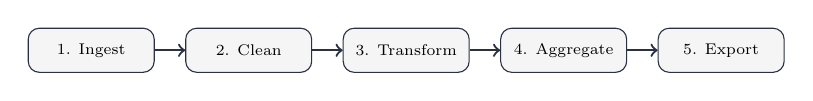
\begin{tikzpicture}[node distance=2cm, scale=0.8, transform shape]
            \tikzstyle{task} = [draw=databricksBlue, fill=databricksLightGray, rounded corners, minimum width=2cm, minimum height=0.7cm, font=\scriptsize]
            \tikzstyle{arrow} = [->, thick, databricksBlue]
            
            \node[task] (ingest) at (0,0) {1. Ingest};
            \node[task] (clean) at (2.5,0) {2. Clean};
            \node[task] (transform) at (5,0) {3. Transform};
            \node[task] (agg) at (7.5,0) {4. Aggregate};
            \node[task] (export) at (10,0) {5. Export};
            
            \draw[arrow] (ingest) -- (clean);
            \draw[arrow] (clean) -- (transform);
            \draw[arrow] (transform) -- (agg);
            \draw[arrow] (agg) -- (export);
        \end{tikzpicture}
    \end{center}
    
    \small Each step depends on the previous one completing successfully!
\end{frame}

% -----------------------------------------------------------------------------
\begin{frame}{Workflow Architecture: Medallion Pipeline}
    \begin{center}
        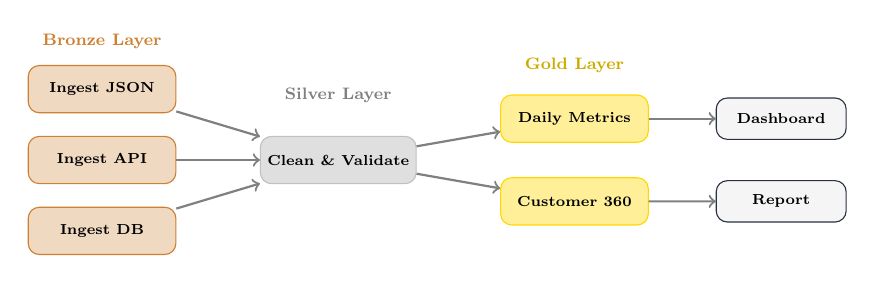
\begin{tikzpicture}[node distance=1.5cm, scale=0.75, transform shape]
            \tikzstyle{bronze} = [draw=bronzeColor, fill=bronzeColor!30, rounded corners, minimum width=2.5cm, minimum height=0.8cm, font=\scriptsize, align=center]
            \tikzstyle{silver} = [draw=silverColor, fill=silverColor!50, rounded corners, minimum width=2.5cm, minimum height=0.8cm, font=\scriptsize, align=center]
            \tikzstyle{gold} = [draw=goldColor, fill=goldColor!40, rounded corners, minimum width=2.5cm, minimum height=0.8cm, font=\scriptsize, align=center]
            \tikzstyle{delivery} = [draw=databricksBlue, fill=databricksLightGray, rounded corners, minimum width=2.2cm, minimum height=0.7cm, font=\scriptsize, align=center]
            \tikzstyle{arrow} = [->, thick, databricksGray]
            
            % Bronze Layer
            \node[bronze] (b1) at (0,0) {\textbf{Ingest JSON}};
            \node[bronze] (b2) at (0,-1.2) {\textbf{Ingest API}};
            \node[bronze] (b3) at (0,-2.4) {\textbf{Ingest DB}};
            
            % Silver Layer
            \node[silver] (s1) at (4,-1.2) {\textbf{Clean \& Validate}};
            
            % Gold Layer
            \node[gold] (g1) at (8,-0.5) {\textbf{Daily Metrics}};
            \node[gold] (g2) at (8,-1.9) {\textbf{Customer 360}};
            
            % Delivery
            \node[delivery] (d1) at (11.5,-0.5) {\textbf{Dashboard}};
            \node[delivery] (d2) at (11.5,-1.9) {\textbf{Report}};
            
            % Arrows
            \draw[arrow] (b1) -- (s1);
            \draw[arrow] (b2) -- (s1);
            \draw[arrow] (b3) -- (s1);
            \draw[arrow] (s1) -- (g1);
            \draw[arrow] (s1) -- (g2);
            \draw[arrow] (g1) -- (d1);
            \draw[arrow] (g2) -- (d2);
            
            % Labels
            \node[font=\footnotesize\bfseries, bronzeColor] at (0,0.8) {Bronze Layer};
            \node[font=\footnotesize\bfseries, databricksGray] at (4,-0.1) {Silver Layer};
            \node[font=\footnotesize\bfseries, goldColor!80!black] at (8,0.4) {Gold Layer};
        \end{tikzpicture}
    \end{center}
\end{frame}

% -----------------------------------------------------------------------------
\begin{frame}{Task Types Available}
    \begin{center}
        \small
        \begin{tabular}{p{2.5cm}|p{4cm}|p{4cm}}
            \toprule
            \rowcolor{databricksBlue}\textcolor{white}{\textbf{Task Type}} & \textcolor{white}{\textbf{Description}} & \textcolor{white}{\textbf{Use Case}} \\
            \midrule
            \textbf{Notebook} & Runs a Databricks notebook & Data transformations, ETL \\
            \rowcolor{databricksLightGray}
            \textbf{Python Script} & Executes Python file & Standalone applications \\
            \textbf{SQL} & Runs SQL queries & Aggregations, transforms \\
            \rowcolor{databricksLightGray}
            \textbf{JAR} & Java/Scala JAR files & Spark applications \\
            \textbf{Delta Live Tables} & DLT pipelines & Declarative ETL \\
            \rowcolor{databricksLightGray}
            \textbf{If/else} & Conditional branching & Dynamic workflow logic \\
            \textbf{For each} & Loop over items & Processing multiple tables \\
            \bottomrule
        \end{tabular}
    \end{center}
\end{frame}

% -----------------------------------------------------------------------------
\begin{frame}{Dependency Patterns}
    \begin{columns}[T]
        \begin{column}{0.32\textwidth}
            \textcolor{databricksBlue}{\textbf{Sequential:}}
            \begin{center}
                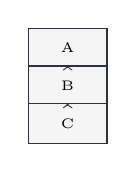
\begin{tikzpicture}[scale=0.6]
                    \tikzstyle{box} = [draw=databricksBlue, fill=databricksLightGray, minimum width=1cm, minimum height=0.5cm, font=\tiny]
                    \node[box] (a) at (0,0) {A};
                    \node[box] (b) at (0,-0.8) {B};
                    \node[box] (c) at (0,-1.6) {C};
                    \draw[->, databricksBlue] (a) -- (b);
                    \draw[->, databricksBlue] (b) -- (c);
                \end{tikzpicture}
            \end{center}
        \end{column}
        \begin{column}{0.32\textwidth}
            \textcolor{databricksBlue}{\textbf{Fan-out (Parallel):}}
            \begin{center}
                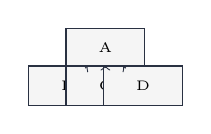
\begin{tikzpicture}[scale=0.6]
                    \tikzstyle{box} = [draw=databricksBlue, fill=databricksLightGray, minimum width=1cm, minimum height=0.5cm, font=\tiny]
                    \node[box] (a) at (0,0) {A};
                    \node[box] (b) at (-0.8,-0.8) {B};
                    \node[box] (c) at (0,-0.8) {C};
                    \node[box] (d) at (0.8,-0.8) {D};
                    \draw[->, databricksBlue] (a) -- (b);
                    \draw[->, databricksBlue] (a) -- (c);
                    \draw[->, databricksBlue] (a) -- (d);
                \end{tikzpicture}
            \end{center}
        \end{column}
        \begin{column}{0.32\textwidth}
            \textcolor{databricksBlue}{\textbf{Fan-in:}}
            \begin{center}
                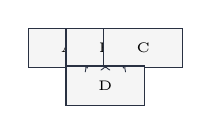
\begin{tikzpicture}[scale=0.6]
                    \tikzstyle{box} = [draw=databricksBlue, fill=databricksLightGray, minimum width=1cm, minimum height=0.5cm, font=\tiny]
                    \node[box] (a) at (-0.8,0) {A};
                    \node[box] (b) at (0,0) {B};
                    \node[box] (c) at (0.8,0) {C};
                    \node[box] (d) at (0,-0.8) {D};
                    \draw[->, databricksBlue] (a) -- (d);
                    \draw[->, databricksBlue] (b) -- (d);
                    \draw[->, databricksBlue] (c) -- (d);
                \end{tikzpicture}
            \end{center}
        \end{column}
    \end{columns}
    
    \vspace{1em}
    \textcolor{databricksBlue}{\textbf{Dependency Conditions:}}
    \begin{itemize}
        \item \textbf{All succeeded} - Run only if ALL upstream tasks completed
        \item \textbf{At least one succeeded} - Run if ANY upstream succeeded
        \item \textbf{None failed} - Run if no upstream failed (includes skipped)
        \item \textbf{All done} - Run regardless of outcomes
    \end{itemize}
\end{frame}

% =============================================================================
% SECTION 4: PARAMETERS AND WIDGETS
% =============================================================================
\begin{frame}{Understanding Parameterization}
    \begin{block}{What is Parameterization?}
        Making code flexible by accepting inputs at runtime rather than hardcoding values.
    \end{block}
    
    \vspace{0.5em}
    \textcolor{databricksBlue}{\textbf{Why Parameterize?}}
    \begin{columns}[T]
        \begin{column}{0.48\textwidth}
            \begin{itemize}
                \item Reuse same notebook for different scenarios
                \item Run pipelines for different dates
            \end{itemize}
        \end{column}
        \begin{column}{0.48\textwidth}
            \begin{itemize}
                \item Test with different configurations
                \item Promote code from dev to prod
            \end{itemize}
        \end{column}
    \end{columns}
    
    \vspace{0.5em}
    \textcolor{databricksBlue}{\textbf{Databricks Widgets}} create input controls that accept values either:
    \begin{itemize}
        \item \textcolor{databricksGreen}{\faCheck} \textbf{Interactively} - in the notebook UI
        \item \textcolor{databricksGreen}{\faCheck} \textbf{Programmatically} - when run as a job
    \end{itemize}
\end{frame}

% -----------------------------------------------------------------------------
\begin{frame}{Widget Types}
    \begin{center}
        \small
        \begin{tabular}{p{2cm}|p{3.5cm}|p{5cm}}
            \toprule
            \rowcolor{databricksBlue}\textcolor{white}{\textbf{Type}} & \textcolor{white}{\textbf{Method}} & \textcolor{white}{\textbf{Best For}} \\
            \midrule
            \textbf{Text} & \texttt{widgets.text()} & File paths, table names, custom strings \\
            \rowcolor{databricksLightGray}
            \textbf{Dropdown} & \texttt{widgets.dropdown()} & Environment selection, layer names \\
            \textbf{Combobox} & \texttt{widgets.combobox()} & Options with occasional custom values \\
            \rowcolor{databricksLightGray}
            \textbf{Multiselect} & \texttt{widgets.multiselect()} & Processing multiple tables/columns \\
            \bottomrule
        \end{tabular}
    \end{center}
\end{frame}

% -----------------------------------------------------------------------------
\begin{frame}[fragile]{Widget Implementation}
    \begin{columns}[T]
        \begin{column}{0.48\textwidth}
            \textcolor{databricksBlue}{\textbf{Creating Widgets:}}
            \begin{lstlisting}[language=Python]
# Text Widget
dbutils.widgets.text(
    "source_path",
    "/mnt/raw/data",
    "Source Data Path"
)

# Dropdown Widget
dbutils.widgets.dropdown(
    "layer",
    "bronze",
    ["bronze", "silver", "gold"],
    "Processing Layer"
)
            \end{lstlisting}
        \end{column}
        \begin{column}{0.48\textwidth}
            \textcolor{databricksBlue}{\textbf{Retrieving Values:}}
            \begin{lstlisting}[language=Python]
# Get single value
source = dbutils.widgets.get(
    "source_path"
)
layer = dbutils.widgets.get(
    "layer"
)

# Multiselect returns comma-
# separated string
tables = dbutils.widgets.get(
    "tables"
).split(",")
            \end{lstlisting}
        \end{column}
    \end{columns}
\end{frame}

% -----------------------------------------------------------------------------
\begin{frame}{Parameter Flow: Interactive vs Job}
    \begin{center}
        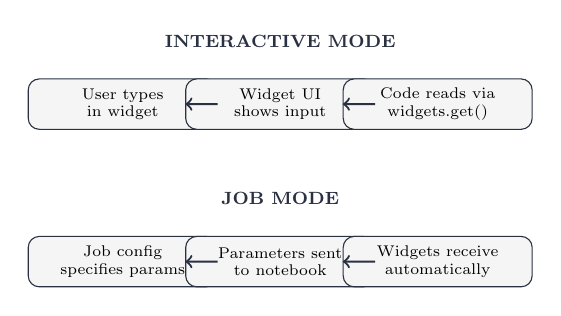
\begin{tikzpicture}[scale=0.8, transform shape]
            \tikzstyle{box} = [draw=databricksBlue, fill=databricksLightGray, rounded corners, minimum width=3cm, minimum height=0.8cm, font=\scriptsize, align=center]
            \tikzstyle{arrow} = [->, thick, databricksBlue]
            
            % Interactive Mode
            \node[font=\footnotesize\bfseries, databricksBlue] at (-4,1.5) {INTERACTIVE MODE};
            \node[box] (i1) at (-6.5,0.5) {User types\\in widget};
            \node[box] (i2) at (-4,0.5) {Widget UI\\shows input};
            \node[box] (i3) at (-1.5,0.5) {Code reads via\\widgets.get()};
            \draw[arrow] (i1) -- (i2);
            \draw[arrow] (i2) -- (i3);
            
            % Job Mode
            \node[font=\footnotesize\bfseries, databricksBlue] at (-4,-1) {JOB MODE};
            \node[box] (j1) at (-6.5,-2) {Job config\\specifies params};
            \node[box] (j2) at (-4,-2) {Parameters sent\\to notebook};
            \node[box] (j3) at (-1.5,-2) {Widgets receive\\automatically};
            \draw[arrow] (j1) -- (j2);
            \draw[arrow] (j2) -- (j3);
        \end{tikzpicture}
    \end{center}
\end{frame}

% =============================================================================
% SECTION 5: SCHEDULING JOBS
% =============================================================================
\begin{frame}{Scheduling Concepts}
    \begin{center}
        \small
        \begin{tabular}{p{2.5cm}|p{4cm}|p{4.5cm}}
            \toprule
            \rowcolor{databricksBlue}\textcolor{white}{\textbf{Type}} & \textcolor{white}{\textbf{Description}} & \textcolor{white}{\textbf{Use Case}} \\
            \midrule
            \textbf{None (Manual)} & Only when manually triggered & Testing, ad-hoc execution \\
            \rowcolor{databricksLightGray}
            \textbf{Scheduled} & Time-based (Cron) & Regular ETL, daily reports \\
            \textbf{Continuous} & Runs continuously, restarts after completion & Real-time/streaming \\
            \rowcolor{databricksLightGray}
            \textbf{File Arrival} & Triggers on new files & Event-driven processing \\
            \bottomrule
        \end{tabular}
    \end{center}
\end{frame}

% -----------------------------------------------------------------------------
\begin{frame}{Cron Expression Format}
    \begin{center}
        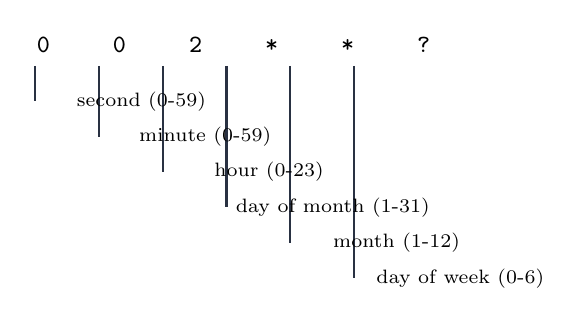
\begin{tikzpicture}[scale=0.9]
            \node[font=\ttfamily\small] at (0,0) {0\hspace{0.8cm}0\hspace{0.8cm}2\hspace{0.8cm}*\hspace{0.8cm}*\hspace{0.8cm}?};
            
            \draw[databricksBlue, thick] (-2.8,-0.3) -- (-2.8,-0.8);
            \draw[databricksBlue, thick] (-1.9,-0.3) -- (-1.9,-1.3);
            \draw[databricksBlue, thick] (-1.0,-0.3) -- (-1.0,-1.8);
            \draw[databricksBlue, thick] (-0.1,-0.3) -- (-0.1,-2.3);
            \draw[databricksBlue, thick] (0.8,-0.3) -- (0.8,-2.8);
            \draw[databricksBlue, thick] (1.7,-0.3) -- (1.7,-3.3);
            
            \node[font=\scriptsize, align=left] at (-1.3,-0.8) {second (0-59)};
            \node[font=\scriptsize, align=left] at (-0.4,-1.3) {minute (0-59)};
            \node[font=\scriptsize, align=left] at (0.5,-1.8) {hour (0-23)};
            \node[font=\scriptsize, align=left] at (1.4,-2.3) {day of month (1-31)};
            \node[font=\scriptsize, align=left] at (2.3,-2.8) {month (1-12)};
            \node[font=\scriptsize, align=left] at (3.2,-3.3) {day of week (0-6)};
        \end{tikzpicture}
    \end{center}
    
    \vspace{0.3em}
    \textcolor{databricksBlue}{\textbf{Common Schedules:}}
    \begin{itemize}
        \item \texttt{0 0 2 * * ?} - Every day at 2:00 AM
        \item \texttt{0 0 * * * ?} - Every hour
        \item \texttt{0 */15 * * * ?} - Every 15 minutes
        \item \texttt{0 0 9 ? * MON-FRI} - Weekdays at 9 AM
    \end{itemize}
\end{frame}

% -----------------------------------------------------------------------------
\begin{frame}{Scheduling Best Practices}
    \begin{columns}[T]
        \begin{column}{0.48\textwidth}
            \textcolor{databricksGreen}{\faCheck\ \textbf{DO:}}
            \begin{itemize}
                \item Avoid peak hours (schedule 2-4 AM)
                \item Stagger similar jobs
                \item Consider dependencies with buffer time
                \item Be explicit about time zones
                \item Monitor execution duration
            \end{itemize}
        \end{column}
        \begin{column}{0.48\textwidth}
            \textcolor{databricksRed}{\faTimes\ \textbf{DON'T:}}
            \begin{itemize}
                \item Schedule all jobs at midnight
                \item Ignore DST transitions
                \item Schedule without buffer time
                \item Forget to set alerts for long-running jobs
            \end{itemize}
        \end{column}
    \end{columns}
\end{frame}

% =============================================================================
% SECTION 6: ERROR HANDLING
% =============================================================================
\begin{frame}{Error Handling: Why It Matters}
    \begin{block}{Production Reality}
        Sources become unavailable, data formats change, clusters run out of memory. Proper error handling ensures \textbf{reliability}, \textbf{visibility}, \textbf{recovery}, and \textbf{debugging}.
    \end{block}
    
    \vspace{0.3em}
    \textcolor{databricksBlue}{\textbf{Types of Failures:}}
    \begin{center}
        \small
        \begin{tabular}{p{2cm}|p{4cm}|p{4cm}}
            \toprule
            \rowcolor{databricksBlue}\textcolor{white}{\textbf{Type}} & \textcolor{white}{\textbf{Examples}} & \textcolor{white}{\textbf{Solution}} \\
            \midrule
            \textbf{Transient} & Network timeout, temp unavailable & Retry automatically \\
            \rowcolor{databricksLightGray}
            \textbf{Resource} & OOM, disk full & Scale up, retry \\
            \textbf{Data} & Schema mismatch, corrupt files & Fix data, alert team \\
            \rowcolor{databricksLightGray}
            \textbf{External} & Source down, API rate limited & Wait and retry \\
            \bottomrule
        \end{tabular}
    \end{center}
\end{frame}

% -----------------------------------------------------------------------------
\begin{frame}{Retry Configuration}
    \begin{columns}[T]
        \begin{column}{0.48\textwidth}
            \textcolor{databricksBlue}{\textbf{Job-Level Retries:}}
            \begin{itemize}
                \item \textbf{Max Retries}: 0-3 recommended
                \item \textbf{Default}: 0 (no retries)
                \item \textbf{Retry on Timeout}: Enable for resource constraints
            \end{itemize}
        \end{column}
        \begin{column}{0.48\textwidth}
            \textcolor{databricksBlue}{\textbf{Task-Level Settings:}}
            \begin{itemize}
                \item \textbf{Max Retries}: 1-3 for most tasks
                \item \textbf{Min Retry Interval}: 30-60 seconds
                \item \textbf{Max Retry Interval}: 300-600 seconds
            \end{itemize}
        \end{column}
    \end{columns}
\end{frame}

% -----------------------------------------------------------------------------
\begin{frame}[fragile]{Error Handling Patterns}
    \textcolor{databricksBlue}{\textbf{Pattern: Exit Codes for Job Control}}
    \begin{lstlisting}[language=Python]
try:
    df = spark.read.format("delta").load("/path/to/data")
    record_count = df.count()
    
    if record_count == 0:
        dbutils.notebook.exit('{"status": "success", "records": 0}')
    
    processed = transform_and_write(df)
    dbutils.notebook.exit(f'{{"status": "success", "records": {processed}}}')
    
except Exception as e:
    error_msg = str(e).replace('"', '\\"')
    dbutils.notebook.exit(f'{{"status": "failed", "error": "{error_msg}"}}')
    raise  # Trigger job retry
    \end{lstlisting}
\end{frame}

% -----------------------------------------------------------------------------
\begin{frame}{Alerting Configuration}
    \begin{center}
        \small
        \begin{tabular}{p{2.5cm}|p{4cm}|p{4cm}}
            \toprule
            \rowcolor{databricksBlue}\textcolor{white}{\textbf{Alert Type}} & \textcolor{white}{\textbf{Trigger}} & \textcolor{white}{\textbf{Notification}} \\
            \midrule
            \textbf{On Failure} & Any task fails (after retries) & Email, Slack, PagerDuty \\
            \rowcolor{databricksLightGray}
            \textbf{On Success} & Job completes successfully & Email (optional) \\
            \textbf{On Duration} & Exceeds expected duration & Monitoring system \\
            \rowcolor{databricksLightGray}
            \textbf{SLA Breach} & Doesn't complete on time & PagerDuty \\
            \bottomrule
        \end{tabular}
    \end{center}
\end{frame}

% =============================================================================
% SECTION 7: BRONZE-SILVER-GOLD PIPELINE
% =============================================================================
\begin{frame}{Bronze Layer: Raw Ingestion}
    \begin{columns}[T]
        \begin{column}{0.55\textwidth}
            \textcolor{bronzeColor}{\textbf{Characteristics:}}
            \begin{itemize}
                \item Raw data as-is from source
                \item Added metadata for lineage
                \item No business transformations
                \item Preserved original schema
            \end{itemize}
            
            \vspace{0.5em}
            \textcolor{databricksBlue}{\textbf{Metadata Added:}}
            \begin{itemize}
                \item \texttt{\_ingestion\_timestamp}
                \item \texttt{\_source\_file}
                \item \texttt{\_process\_date}
                \item \texttt{\_row\_hash} (SHA-256)
            \end{itemize}
        \end{column}
        \begin{column}{0.42\textwidth}
            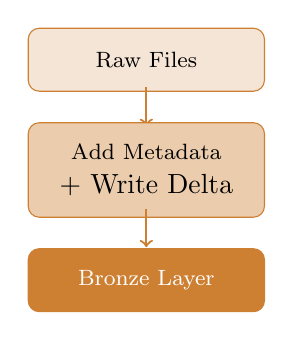
\begin{tikzpicture}[scale=0.7]
                \node[draw=bronzeColor, fill=bronzeColor!20, rounded corners, minimum width=3cm, minimum height=0.8cm] (source) at (0,2) {\footnotesize Raw Files};
                \draw[->, thick, bronzeColor] (0,1.5) -- (0,0.8);
                \node[draw=bronzeColor, fill=bronzeColor!40, rounded corners, minimum width=3cm, minimum height=1.2cm, align=center] (process) at (0,0) {\footnotesize Add Metadata\\+ Write Delta};
                \draw[->, thick, bronzeColor] (0,-0.7) -- (0,-1.4);
                \node[draw=bronzeColor, fill=bronzeColor, text=white, rounded corners, minimum width=3cm, minimum height=0.8cm] (bronze) at (0,-2) {\footnotesize Bronze Layer};
            \end{tikzpicture}
        \end{column}
    \end{columns}
\end{frame}

% -----------------------------------------------------------------------------
\begin{frame}{Silver Layer: Cleansed Data}
    \begin{columns}[T]
        \begin{column}{0.55\textwidth}
            \textcolor{databricksGray}{\textbf{Characteristics:}}
            \begin{itemize}
                \item Cleaned and validated data
                \item Standardized formats
                \item Deduplication applied
                \item Schema enforced
                \item Data quality checks passed
            \end{itemize}
            
            \vspace{0.3em}
            \textcolor{databricksBlue}{\textbf{Quality Rules:}}
            \begin{itemize}
                \item Remove nulls in required fields
                \item Standardize strings (trim)
                \item Remove duplicates
                \item Validate value ranges
            \end{itemize}
        \end{column}
        \begin{column}{0.42\textwidth}
            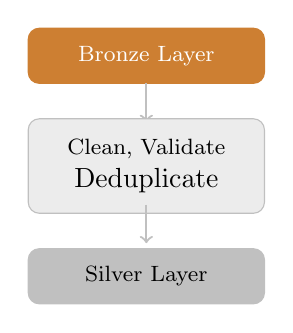
\begin{tikzpicture}[scale=0.7]
                \node[draw=bronzeColor, fill=bronzeColor, text=white, rounded corners, minimum width=3cm, minimum height=0.7cm] (bronze) at (0,2) {\footnotesize Bronze Layer};
                \draw[->, thick, silverColor] (0,1.5) -- (0,0.8);
                \node[draw=silverColor, fill=silverColor!30, rounded corners, minimum width=3cm, minimum height=1.2cm, align=center] (process) at (0,0) {\footnotesize Clean, Validate\\Deduplicate};
                \draw[->, thick, silverColor] (0,-0.7) -- (0,-1.4);
                \node[draw=silverColor, fill=silverColor, rounded corners, minimum width=3cm, minimum height=0.7cm] (silver) at (0,-2) {\footnotesize Silver Layer};
            \end{tikzpicture}
        \end{column}
    \end{columns}
\end{frame}

% -----------------------------------------------------------------------------
\begin{frame}{Gold Layer: Business Aggregations}
    \begin{columns}[T]
        \begin{column}{0.55\textwidth}
            \textcolor{goldColor!80!black}{\textbf{Aggregation Types:}}
            \begin{itemize}
                \item \textbf{Daily Summary}: Totals by category
                \item \textbf{Customer Metrics}: Lifetime value, segmentation
                \item \textbf{Product Performance}: Revenue rankings
                \item \textbf{Regional Analysis}: Revenue by region
            \end{itemize}
            
            \vspace{0.3em}
            \textcolor{databricksBlue}{\textbf{Customer Segments:}}
            \begin{itemize}
                \item Platinum: LTV $\geq$ \$10,000
                \item Gold: LTV $\geq$ \$5,000
                \item Silver: LTV $\geq$ \$1,000
                \item Bronze: LTV $<$ \$1,000
            \end{itemize}
        \end{column}
        \begin{column}{0.42\textwidth}
            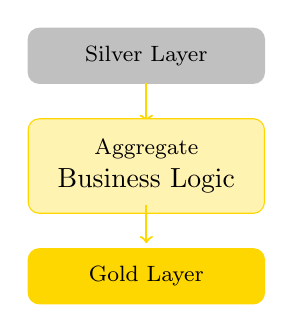
\begin{tikzpicture}[scale=0.7]
                \node[draw=silverColor, fill=silverColor, rounded corners, minimum width=3cm, minimum height=0.7cm] (silver) at (0,2) {\footnotesize Silver Layer};
                \draw[->, thick, goldColor] (0,1.5) -- (0,0.8);
                \node[draw=goldColor, fill=goldColor!30, rounded corners, minimum width=3cm, minimum height=1.2cm, align=center] (process) at (0,0) {\footnotesize Aggregate\\Business Logic};
                \draw[->, thick, goldColor] (0,-0.7) -- (0,-1.4);
                \node[draw=goldColor, fill=goldColor, rounded corners, minimum width=3cm, minimum height=0.7cm] (gold) at (0,-2) {\footnotesize Gold Layer};
            \end{tikzpicture}
        \end{column}
    \end{columns}
\end{frame}

% -----------------------------------------------------------------------------
\begin{frame}{Job Configuration: Daily ETL Pipeline}
    \begin{columns}[T]
        \begin{column}{0.48\textwidth}
            \textcolor{databricksBlue}{\textbf{General Settings:}}
            \begin{itemize}
                \item \textbf{Job Name}: daily\_etl\_pipeline
                \item \textbf{Max Concurrent}: 1
                \item \textbf{Timeout}: 4 hours
            \end{itemize}
            
            \vspace{0.3em}
            \textcolor{databricksBlue}{\textbf{Schedule:}}
            \begin{itemize}
                \item \textbf{Cron}: 0 0 2 * * ?
                \item \textbf{Time Zone}: America/New\_York
                \item Daily at 2:00 AM Eastern
            \end{itemize}
        \end{column}
        \begin{column}{0.48\textwidth}
            \textcolor{databricksBlue}{\textbf{Cluster Config:}}
            \begin{itemize}
                \item \textbf{Workers}: 2-8 (autoscaling)
                \item \textbf{Spark}: 12.2.x-scala2.12
                \item \textbf{Auto-terminate}: 10 min
            \end{itemize}
            
            \vspace{0.3em}
            \textcolor{databricksBlue}{\textbf{Alerts:}}
            \begin{itemize}
                \item On Failure: Email team
                \item On Duration $>$ 2h: Warn team
            \end{itemize}
        \end{column}
    \end{columns}
\end{frame}

% =============================================================================
% SECTION 8: BEST PRACTICES
% =============================================================================
\begin{frame}{Job Design Best Practices}
    \begin{center}
        \small
        \begin{tabular}{p{2.5cm}|p{4cm}|p{4.5cm}}
            \toprule
            \rowcolor{databricksBlue}\textcolor{white}{\textbf{Category}} & \textcolor{white}{\textbf{Best Practice}} & \textcolor{white}{\textbf{Rationale}} \\
            \midrule
            \textbf{Idempotency} & Safely re-runnable & Retry without data corruption \\
            \rowcolor{databricksLightGray}
            \textbf{Parameterize} & Use params for env values & Same code in dev/staging/prod \\
            \textbf{Small Tasks} & Break into focused tasks & Easier debugging, parallelism \\
            \rowcolor{databricksLightGray}
            \textbf{Logging} & Meaningful log messages & Aid troubleshooting \\
            \textbf{Exit Codes} & Use notebook.exit() & Enable downstream decisions \\
            \rowcolor{databricksLightGray}
            \textbf{Checkpoints} & Save progress periodically & Recovery without restart \\
            \bottomrule
        \end{tabular}
    \end{center}
\end{frame}

% -----------------------------------------------------------------------------
\begin{frame}{Cluster \& Scheduling Best Practices}
    \begin{columns}[T]
        \begin{column}{0.48\textwidth}
            \textcolor{databricksBlue}{\textbf{Cluster Configuration:}}
            \begin{itemize}
                \item Use \textbf{Job Clusters} for production
                    \begin{itemize}
                        \item \textcolor{databricksRed}{$\triangleright$} Cost-efficient, isolated
                    \end{itemize}
                \item Enable \textbf{Autoscaling}
                    \begin{itemize}
                        \item \textcolor{databricksRed}{$\triangleright$} Min 2, max based on volume
                    \end{itemize}
                \item Use \textbf{Spot Instances}
                    \begin{itemize}
                        \item \textcolor{databricksRed}{$\triangleright$} 60-90\% cost reduction
                    \end{itemize}
                \item Use \textbf{LTS Spark versions}
            \end{itemize}
        \end{column}
        \begin{column}{0.48\textwidth}
            \textcolor{databricksBlue}{\textbf{Scheduling Tips:}}
            \begin{itemize}
                \item Avoid scheduling at midnight
                \item Use buffer time between jobs
                \item Be explicit about time zones
                \item Set duration alerts
                \item Stagger similar jobs
            \end{itemize}
        \end{column}
    \end{columns}
\end{frame}

% =============================================================================
% SECTION 9: TROUBLESHOOTING
% =============================================================================
\begin{frame}{Troubleshooting Common Issues}
    \textcolor{databricksBlue}{\textbf{Issue 1: Job Fails to Start}}
    \begin{itemize}
        \item \textbf{Causes}: Quota exceeded, no capacity, invalid config, permissions
        \item \textbf{Solution}: Check quotas, try different region/instance type
    \end{itemize}
    
    \vspace{0.3em}
    \textcolor{databricksBlue}{\textbf{Issue 2: Task Timeout}}
    \begin{itemize}
        \item \textbf{Diagnostic}: Check data volume, Spark UI, data skew
        \item \textbf{Solution}: Increase timeout, optimize queries, add workers
    \end{itemize}
    
    \vspace{0.3em}
    \textcolor{databricksBlue}{\textbf{Issue 3: Parameter Not Passed}}
    \begin{itemize}
        \item \textbf{Cause}: Parameter name mismatch between notebook and job
        \item \textbf{Solution}: Ensure exact name match (case-sensitive)
    \end{itemize}
\end{frame}

% -----------------------------------------------------------------------------
\begin{frame}[fragile]{Troubleshooting: Retries Not Working}
    \textcolor{databricksBlue}{\textbf{Common Causes:}}
    \begin{itemize}
        \item \texttt{notebook.exit()} called with error status (counts as success!)
        \item Exception not raised after exit
        \item Retry configured at wrong level
    \end{itemize}
    
    \vspace{0.3em}
    \textcolor{databricksGreen}{\textbf{Correct Pattern:}}
    \begin{lstlisting}[language=Python]
try:
    result = process_data()
    dbutils.notebook.exit(f'{{"status": "success", "count": {result}}}')
except Exception as e:
    print(f"ERROR: {str(e)}")
    dbutils.notebook.exit(f'{{"status": "failed", "error": "{str(e)}"}}')
    raise  # IMPORTANT: Raise to trigger retry!
    \end{lstlisting}
\end{frame}

% =============================================================================
% SUMMARY
% =============================================================================
\begin{frame}{Key Takeaways}
    \begin{columns}[T]
        \begin{column}{0.48\textwidth}
            \textcolor{databricksBlue}{\textbf{Core Concepts:}}
            \begin{enumerate}
                \item \textbf{Jobs vs Notebooks}: Dev vs Production
                \item \textbf{Multi-Task Workflows}: Chain with dependencies
                \item \textbf{Parameters}: Widgets for flexibility
                \item \textbf{Scheduling}: Cron expressions
            \end{enumerate}
        \end{column}
        \begin{column}{0.48\textwidth}
            \textcolor{databricksBlue}{\textbf{Production Patterns:}}
            \begin{enumerate}
                \item \textbf{Error Handling}: Retries \& alerts
                \item \textbf{Medallion}: Bronze$\rightarrow$Silver$\rightarrow$Gold
                \item \textbf{Idempotency}: Safe to re-run
                \item \textbf{Monitoring}: Track \& alert
            \end{enumerate}
        \end{column}
    \end{columns}
\end{frame}

% -----------------------------------------------------------------------------
\begin{frame}{Implementation Checklist}
    \begin{columns}[T]
        \begin{column}{0.48\textwidth}
            \begin{itemize}
                \item[$\square$] Parameterize notebooks with widgets
                \item[$\square$] Create separate notebooks per layer
                \item[$\square$] Set up multi-task job with dependencies
                \item[$\square$] Configure retry settings
            \end{itemize}
        \end{column}
        \begin{column}{0.48\textwidth}
            \begin{itemize}
                \item[$\square$] Set up failure alerting
                \item[$\square$] Schedule at appropriate time
                \item[$\square$] Test end-to-end with sample data
                \item[$\square$] Document the pipeline
            \end{itemize}
        \end{column}
    \end{columns}
    
    \vspace{1em}
    \begin{center}
        \textcolor{databricksGreen}{\Large\faCheckCircle\ Ready to build production pipelines!}
    \end{center}
\end{frame}

% -----------------------------------------------------------------------------
% THANK YOU SLIDE
% -----------------------------------------------------------------------------
\begin{frame}[plain]
    \begin{tikzpicture}[remember picture,overlay]
        \fill[databricksBlue] (current page.north west) rectangle (current page.south east);
    \end{tikzpicture}
    \begin{center}
        \vspace{2cm}
        {\Huge\textcolor{databricksWhite}{\textbf{Thank You!}}}
        
        \vspace{1cm}
        {\large\textcolor{databricksYellow}{Day 7: Databricks Jobs \& Workflows}}
        
        \vspace{1.5cm}
        {\textcolor{databricksLightGray}{
            \faLinkedin\ \href{https://www.linkedin.com/in/yashkavaiya}{linkedin.com/in/yashkavaiya}\\[0.3em]
            \faGlobe\ \href{https://easy-ai-labs.lovable.app/}{easy-ai-labs.lovable.app}\\[0.3em]
            \faBuilding\ \href{https://www.linkedin.com/company/genai-guru}{Gen AI Guru}
        }}
    \end{center}
\end{frame}

\end{document}
